\subsection{Kiểm chứng độ tin cậy của thuật toán}

Kết quả tính toán quỹ đạo chuyển động của vật thể trong trường trọng lực với vận tốc ban đầu \(v_0 = \qty{50}{\meter\per\second}\), tại các góc bắn khác nhau, được thực hiện bằng phương pháp Runge-Kutta (RK4).

Để kiểm chứng độ chính xác của chương trình, trước hết tiến hành mô phỏng trong điều kiện lý tưởng (\(k = 0\)) và so sánh với lời giải giải tích truyền thống.

\begin{table*}[t]
    \centering
    \begin{tabular}{@{}llccc@{}}
      \toprule
      \textbf{Thông số} & \textbf{Phương pháp} & \textbf{30$^\circ$} & \textbf{45$^\circ$} & \textbf{60$^\circ$} \\
      \midrule
      % data/latex_table.tex
      \multirow{3}{*}{\(H_{\max}\) (\unit{\meter})}
                        & Kết quả RK4   & \num{509.683995}  & \num{1019.367992}  & \num{1529.051985} \\
                        & Lý thuyết     & \num{509.683996}  & \num{1019.367992}  & \num{1529.051988} \\
                        & Sai số tỷ đối & \num{1.000000}  & \num{1.000000}  & \num{1.000000} \\
      \midrule
      \multirow{3}{*}{\(R\) (\unit{\meter})}
                        & Kết quả RK4   & \num{3531.353135}  & \num{4077.407741}  & \num{3531.353135} \\
                        & Lý thuyết     & \num{3531.194307}  & \num{4077.471967}  & \num{3531.194307} \\
                        & Sai số tỷ đối & \num{1.000045}  & \num{0.999984}  & \num{1.000045} \\
      \bottomrule
    \end{tabular}
    \caption{So sánh kết quả phương RK4 với kết quả giải tích (\(v_0 = \qty{200}{\meter\per\second}, \alpha = \qty{30}{\degree},\qty{45}{\degree},\qty{60}{\degree}, N = 500\))}\label{tab:kiem_chung}
\end{table*}

Các số liệu ở Bảng \ref{tab:kiem_chung} cho thấy sự tương đồng rất cao giữa kết quả mô phỏng và lý thuyết vật lý cổ điển. Điều này chứng tỏ thuật toán RK4 là đủ chính xác và đáng tin cậy để áp dụng cho các trường hợp phức tạp hơn có lực cản không khí.

\subsection{Ảnh hưởng của lực cản tới quỹ đạo}

Khi xét đến lực cản không khí, quỹ đạo chuyển động của vật thể không còn giữ được hình dạng parabol đối xứng hoàn hảo như trong môi trường chân không. Các kết quả mô phỏng cho thấy lực cản tác động rõ rệt lên mọi thông số đặc trưng của chuyển động.

Từ Hình~\ref{fig:1}, có thể thấy rõ hiện tượng quỹ đạo bị ép ngắn lại. Điểm rơi của vật thể gần vị trí bắn hơn và đỉnh cao nhất của quỹ đạo cũng thấp hơn đáng kể.

\begin{figure}[H]
    \centering
    \begin{minipage}[t]{\linewidth}
        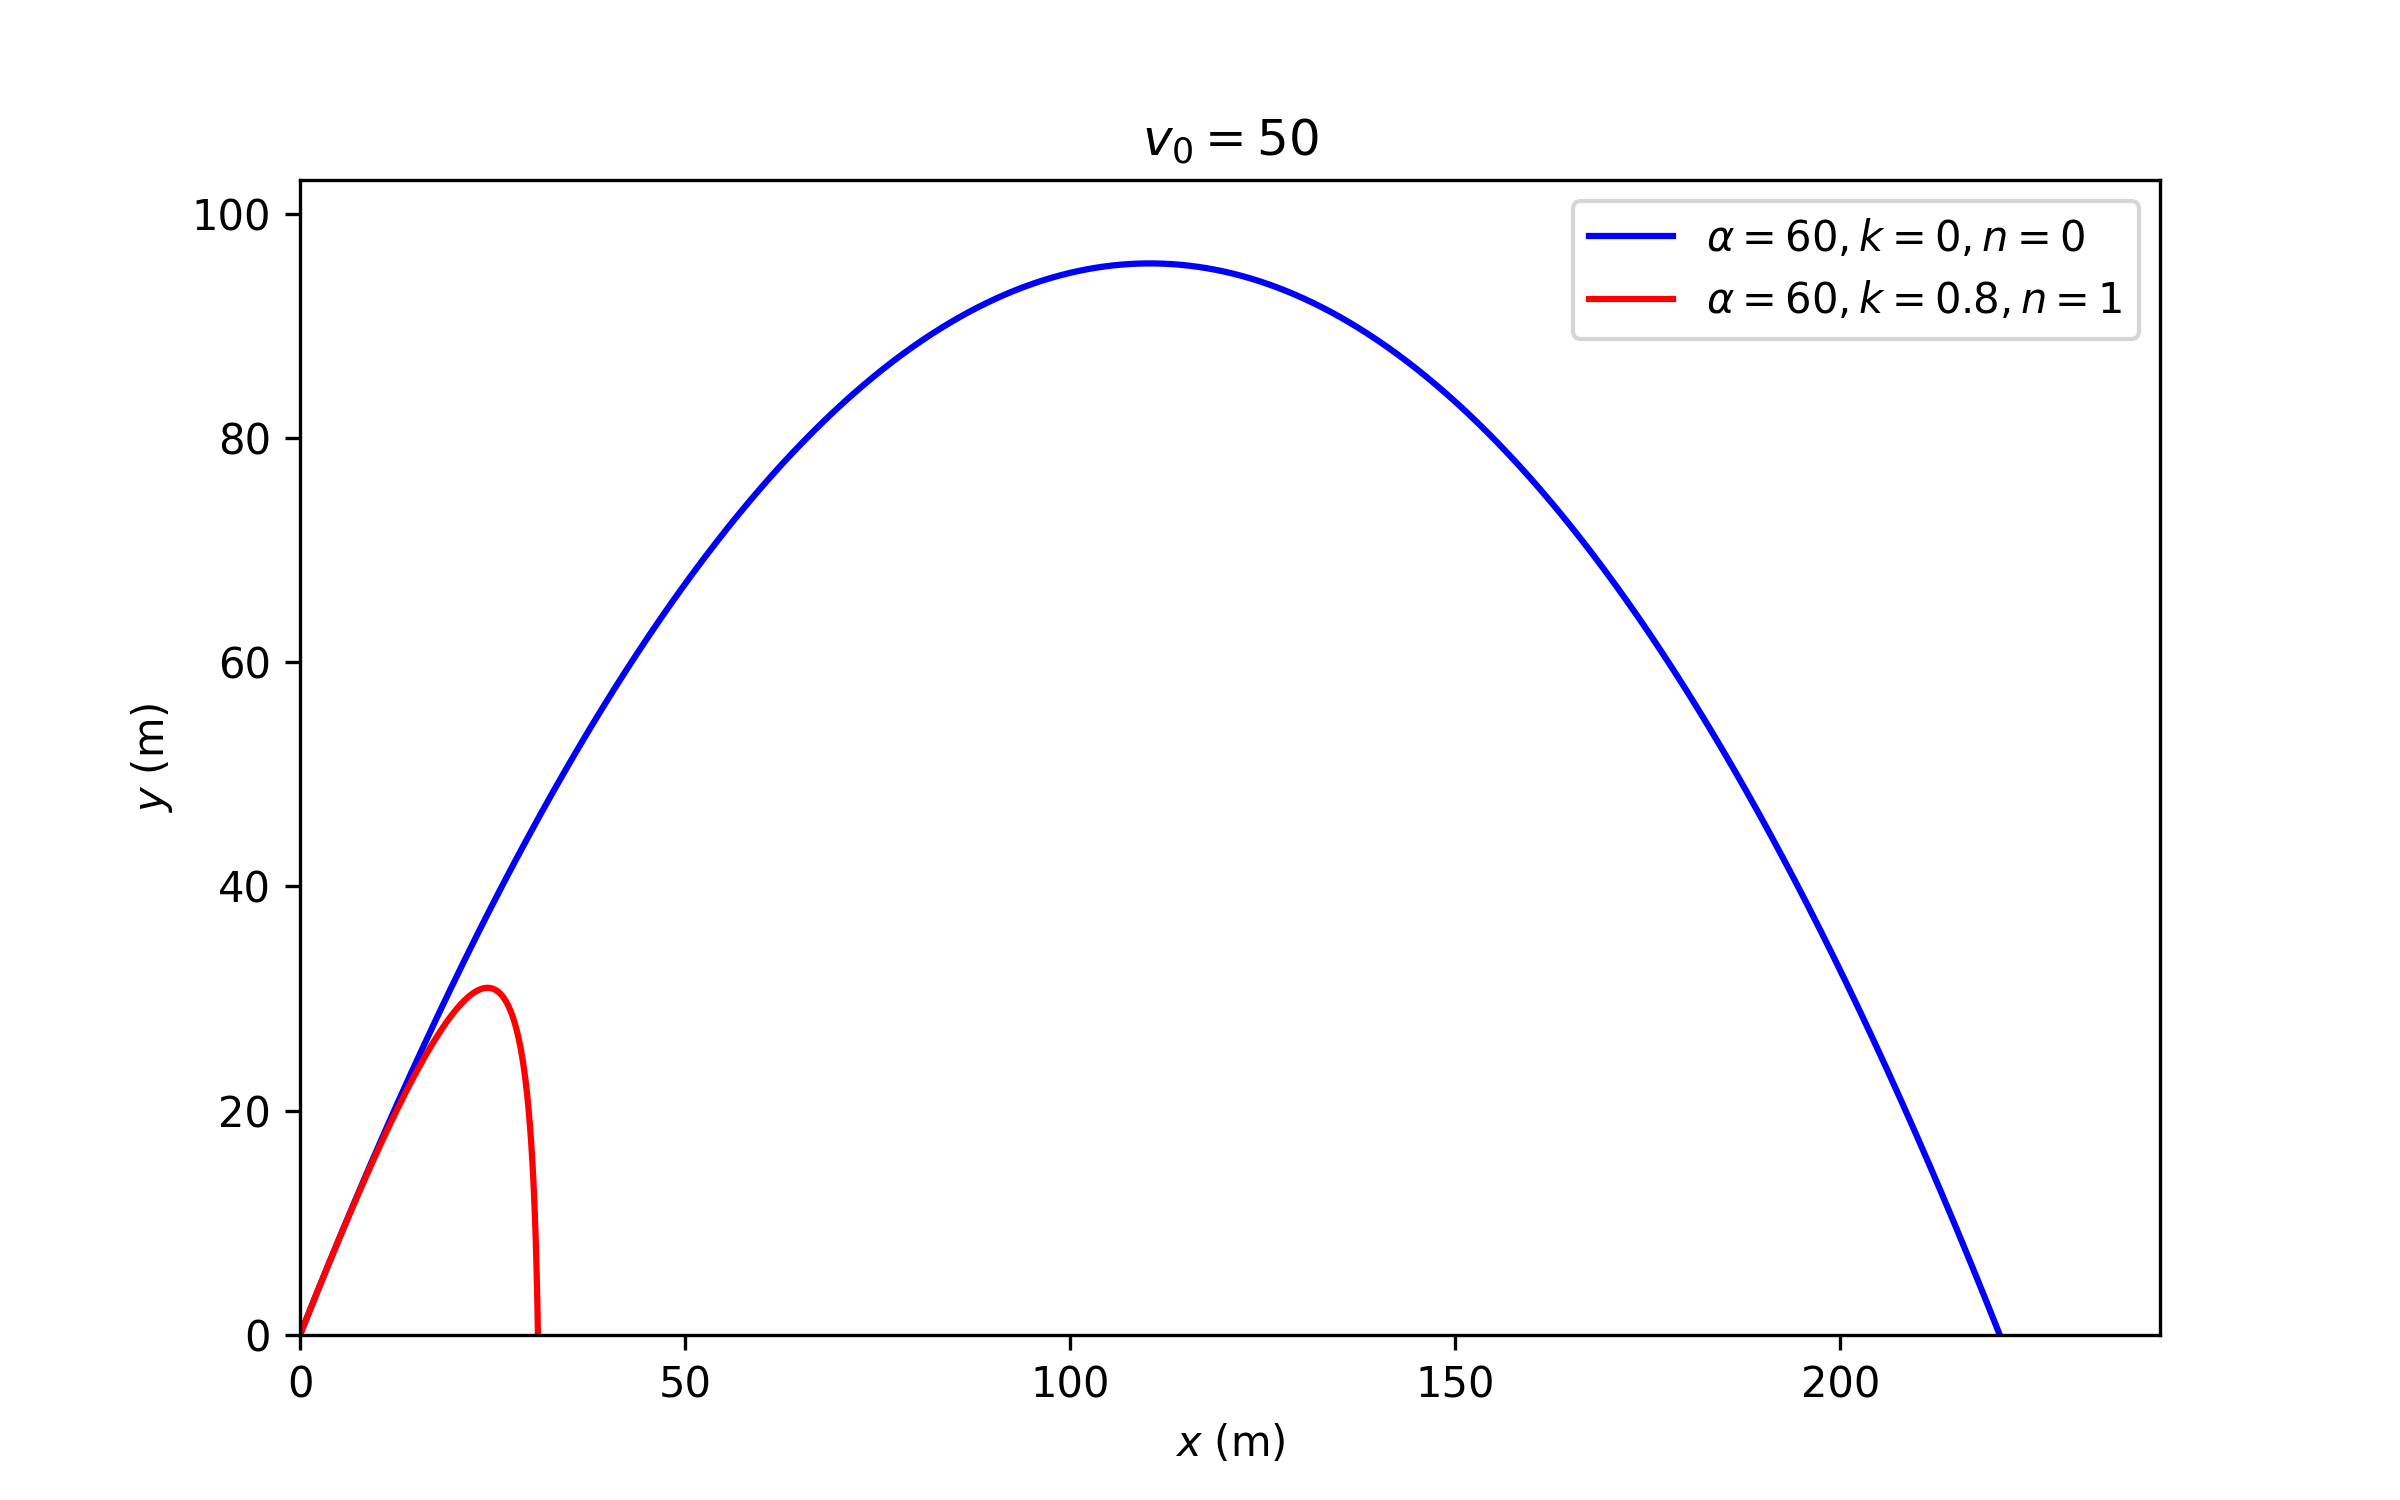
\includegraphics[width=\linewidth]{images/drag_vs_nodrag.png}
        \caption{So sánh quỹ đạo trong chân không và quỹ đạo khi có lực cản không khí}\label{fig:1}
    \end{minipage}
    \begin{minipage}[t]{\linewidth}
        
\includegraphics[width=\linewidth]{drag_exponent.png}
        \caption{Ảnh hưởng của số mũ lực cản đến hình dạng quỹ đạo}
    \end{minipage}
\end{figure}

\subsection{Ảnh hưởng của thông số lực cản tới quỹ đạo}

Nghiên cứu tiến hành khảo sát sự thay đổi của quỹ đạo khi hệ số cản $k = 0,8$ và bậc lũy thừa $n$ bằng 1, 1.5 và 2. Kết quả chi tiết được trình bày trong Bảng~\ref{tab:anh_huong_luc_can} và Biểu diễn qua Hình~\ref{fig:3} và \ref{fig:4}.

\begin{figure}[H]
    \centering
    \begin{minipage}[t]{\linewidth}
        
\includegraphics[width=\linewidth]{drag_angle.png}
        \caption{Ảnh hưởng của góc bắn tới tầm xa}\label{fig:3}
    \end{minipage}
    \begin{minipage}[t]{\linewidth}
        
\includegraphics[width=\linewidth]{drag_velocity.png}
        \caption{Ảnh hưởng của vận tốc đầu tới tầm xa}\label{fig:4}
    \end{minipage}
\end{figure}

\begin{table*}[t]
    \centering
    \begin{tabular}{@{}ccccc@{}}
      \toprule
      \textbf{Hệ số $n$} & \textbf{Góc bắn ($^\circ$)} & \textbf{Tầm xa ($R$, m)} & \textbf{Độ cao ($H_{\max}$, m)} & \textbf{Thời gian ($T$, s)} \\ \midrule
      $n = 1$ & 30 & 50,42 & 10,25 & 2,74 \\
      (Tuyến tính) & 45 & 47,88 & 17,31 & 3,75 \\
                         & 60 & 40,24 & 22,81 & 4,49 \\ \midrule
      $n = 1,5$ & 30 & 25,18 & 6,34 & 1,84 \\
                         & 45 & 22,76 & 10,21 & 2,49 \\
                         & 60 & 18,52 & 13,06 & 2,93 \\ \midrule
      $n = 2$ & 30 & 14,02 & 4,12 & 1,36 \\
      (Bình phương) & 45 & 12,41 & 6,42 & 1,81 \\
                         & 60 & 9,96 & 8,05 & 2,12 \\ \bottomrule
    \end{tabular}
    \caption{Thông số quỹ đạo dưới ảnh hưởng của lực cản ($k=0,8, v_0=50$ m/s)}
    \label{tab:anh_huong_luc_can}
\end{table*}
